We evaluate our intersection of unions method on two real world
examples, i.e., a $7$-dimensional nonlinear model of an autonomous car
from Lavaei et. al.~\cite{lavaei2020formal} and a $12$-dimensional
nonlinear model of a quadrotor from ARCH 2020
workshop~\cite{geretti2020arch}.  On these examples, besides the union
method based on the performance index~(\ref{eqn:pi}) proposed in
Althoff et. al.~\cite{althoff2008reachability}, we compare with
with polynomial zonotopes~\cite{althoff2013reachability} in CORA
tool\footnote{\url{https://tumcps.github.io/CORA}} and Taylor
models~\cite{chen2012taylor} in
Flowstar\footnote{https://flowstar.org}.

For computation of symbolic derivatives, we use Sympy Python
software~\cite{10.7717/peerj-cs.103} and for interval arithmetic, we
use Boost C++ library~\cite{bronnimann2006design}.  We use
OpenMp\footnote{\url{https://www.openmp.org}} to run in
parallel each iteration Step~\ref{step:1} of the for loops of
Algorithm~\ref{alg:main}.
\is{Algorithm 2 has othe (in parallel) steps. Should we remove those?}

\emph{Settings:}  We
ran our IoU method, union method and Flowstar Taylor model on an AWS
c5a.16xlarge cluster with 64 virtual CPU cores.  We ran CORA in MATLAB
2019a on a 1.4GHz laptop with 4GB 1600MHz DDR3 RAM.  The
simulation time step is $\delta = 0.005\si{\second}$ for car model and
$\delta = 0.01\si{\second}$ for quadrotor model.  The simulation time
horizon is $[0, 5\si{\second}]$.  The order of Taylor expansion of
Flowstar Taylor model is $9$ for car model and $7$ for quadrotor
model.  For the CORA polynomial zonotope, our IoU method and the union
method, the generator order is $l=400$ for car model and $l=200$ for
quadrotor model.  The order of \emph{dependent generators} of
polynomial zonotope is $2000$ for both models.  We took $K = 20$ and
$\epsilon = 10^{-12}$.  For the union method, the normalization error
$\rho$ for division~(Equation~\ref{eqn:pi}) is $\rho
= \taylor{f}{X_0}{u}$, i.e., the Taylor error before division.

%% \subsection{Illustrative example: IoU  vs union of interval zonotopes}
%% We consider the 3-dimensional nonlinear system in Example~\ref{eg:ill}
%% \is{Does it represent some real system, for example, a bicycle? It would have been nice then.}
%% to illustrate the difference in accuracy between our IoU flowpipe and
%% the union flowpipe based on the performance index
%% in~\cite{althoff2008reachability}(Equation~\ref{eqn:pi} above).  The
%% initial set has to be large enough to demonstrate the effect of linearization error, which is $X_0 = [-1,1]^3$.

%% \emph{Settings:}  We ran both the IoU and unions algorithm on a 1.4 GHz
%% laptop with 4 GB ram, 1600 MHz DDR3 with 4 virtual cpu cores.
%% \is{If you are usimg the same machine configuration for all the experiments, then the above line should move before Section 4.1}
%% We consider $3$ different number of divisions for comparision, i.e.,
%% $2^\eta:\eta = 2, 3,4$, or $4, 8$ and $16$ divisions,
%% respectively. The order of interval zonotope is $l = 200$ and the time
%% step size is $\delta = 0.01\si{\second}$.  Furthermore, $\epsilon = 10^{-12}$
%% and $K = 20$.  The normalization error $\rho$ for division in the union method is
%% the Taylor error before splitting $\taylor{f}{X_0}{U}$.

%% \emph{Results:}  The upper and lower bounds on flowpipes at uniformly spaced time
%% points for the $x$ and $y$ variables is
%% shown in Figure~\ref{fig:ill}. 
%% The figure clearly demonstrates that our IoU
%% flowpipe is far more accurate than the union flowpipe for $x/y$
%% coordinates.  The bounds for $\theta$ are almost similar for both
%% methods and all types of divisions because of very less linearization
%% error $(\le 10^{-6})$.  The computation times for our IoU method are $6\si{\second}$, $12\si{\second}$ and $24\si{\second}$, respectively, for $4$, $8$ and $16$ divisions
%% per union.  The computation times will reduce significantly by using
%% more cpu cores.  We use more cpu cores for the higher dimensional
%% examples that we evaluate latter.
%% \is{The parallel computation aspect needs more details. May be in the Algorithm section, you may say how to parallelize your algorithm.}
%% %
\begin{figure}
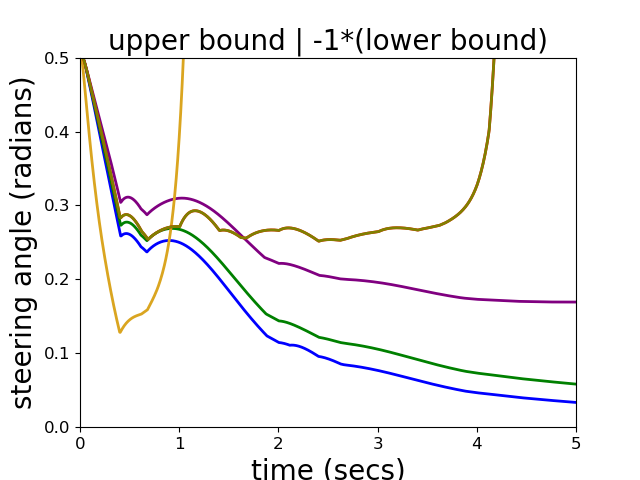
\includegraphics[scale = 0.39]{autocarImages/ubToolSteering.png}\hspace{-2.2em}
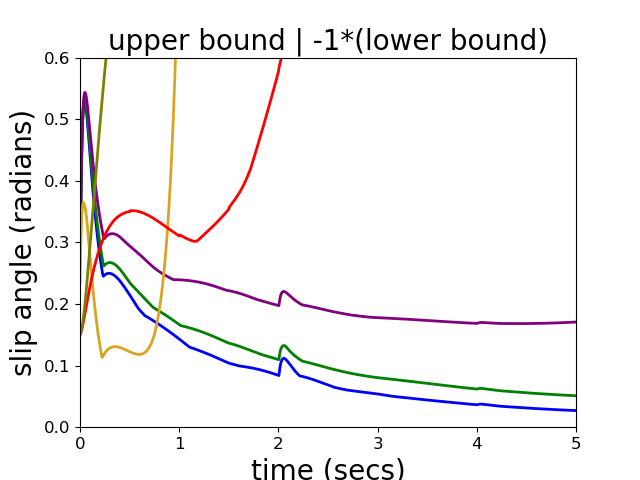
\includegraphics[scale = 0.39]{autocarImages/ubToolSlip.png}
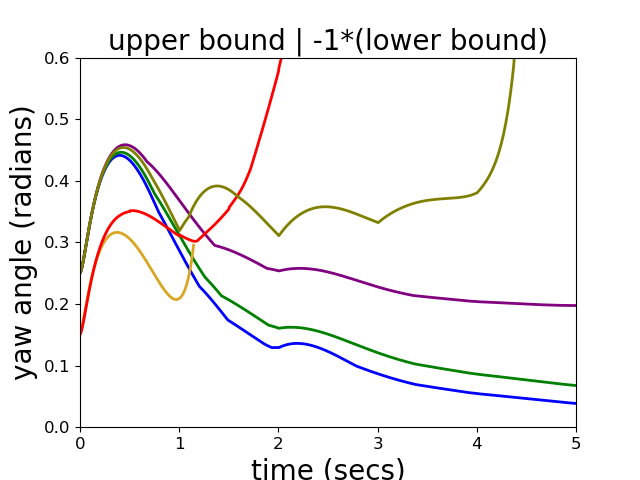
\includegraphics[scale = 0.39]{autocarImages/ubToolYaw.png}\hspace{-2.2em}
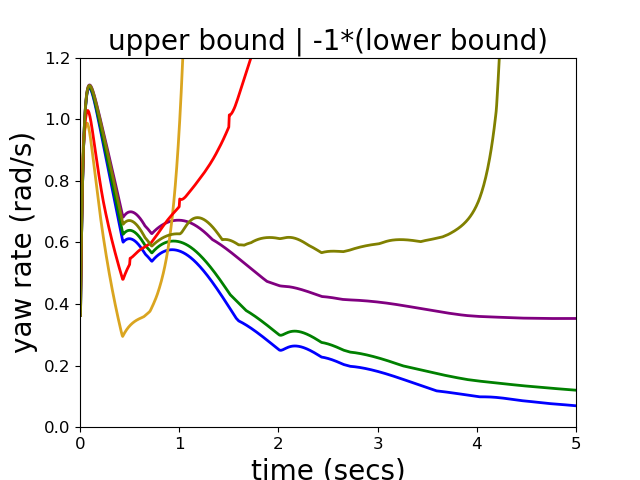
\includegraphics[scale = 0.39]{autocarImages/ubToolYawRate.png}
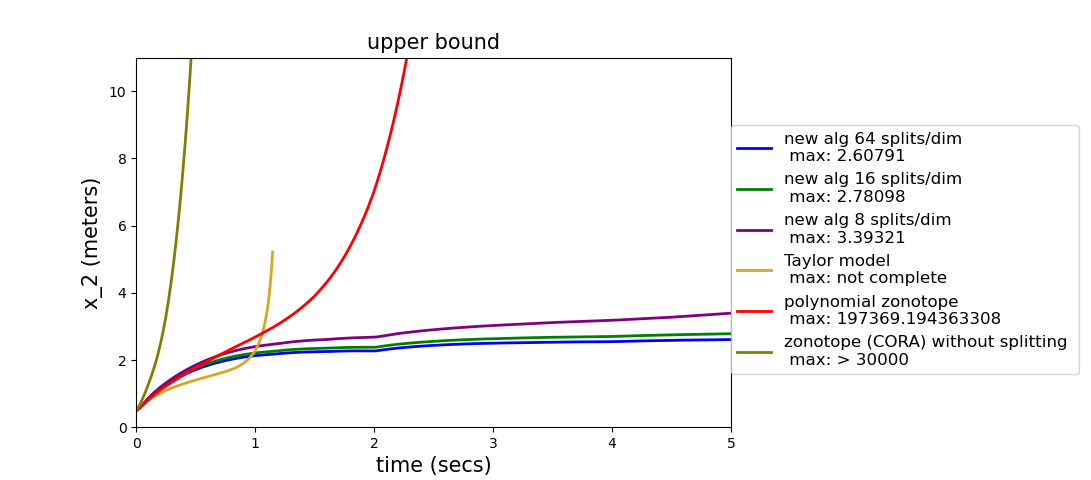
\includegraphics[scale = 0.41]{autocarImages/ubToolx2.png}\hspace{-2.2em}
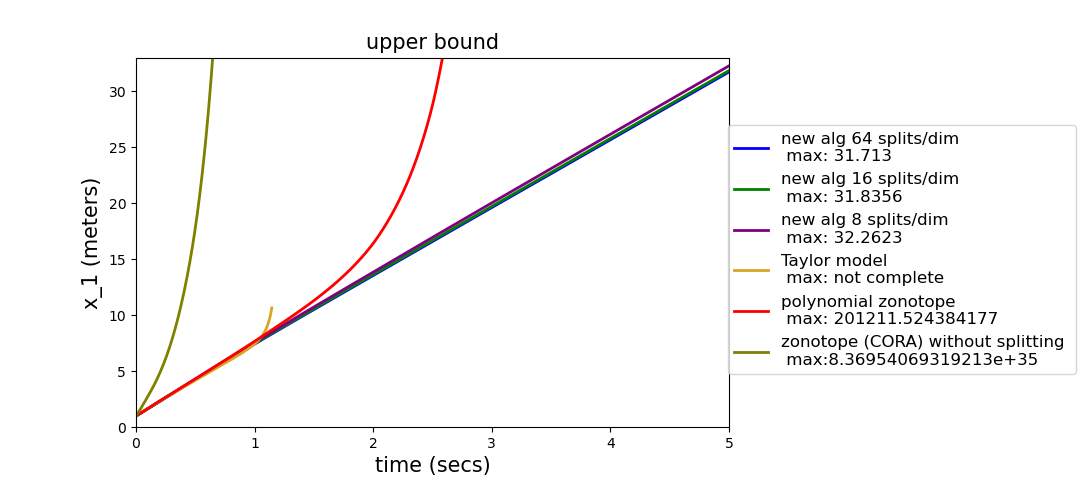
\includegraphics[scale = 0.39]{autocarImages/ubToolx1.png}

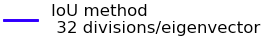
\includegraphics[scale = 0.41]{autocarImages/leg1.png}~
  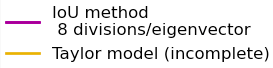
\includegraphics[scale = 0.41]{autocarImages/leg2.png}~
  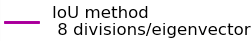
\includegraphics[scale = 0.41]{autocarImages/leg3.png}
  \caption{Flowpipe bounds at different time points for
    car model}\label{fig:flowcar}
\end{figure}
%
\subsection{$7$-dimensional model of autonomous car}
A time discretized model of autonomous car manoeuvre with $7$-dimensional
state space and $2$ inputs was presented in~\cite{lavaei2020formal}.
We adapted this model into a continuous time system and provided a
stabilizing feedback with one of the inputs.  Then we have the
following $7$-dimensional system having only one
uncontrolled input.
%
\begin{align*}
\dot{x_1}  = & x_4\cos\rb{x_5+x_7}\hspace{2em} \dot{x_2} =
x_4\sin\rb{x_5+x_7}\\
%
\dot{x_3}  = & -r(x_5+x_7+x_3) \hspace{2em} \dot{x_4} =
 u \hspace{2em} \dot{x_5} = x_6 & \\
 %
 \dot{x_6}  = & \frac{\mu
 m}{I_z(l_r+l_f)}(l_fC_{Sf}(gl_r-uh_{cg})x_3+
 (l_rC_{Sr}(gl_f+uh_{cg})\\& -l_fC_{Sf}(gl_r-uh_{cg}))x_7
 -(l_fl_fC_{Sf}(gl_r-uh_{cg}) + l_rl_rC_{Sr}(gl_f+uh_{cg}))\frac{x_6}{x_4})\\
%
\dot{x_7} 
= & \frac{\mu}{x_4(l_r+l_f)}(C_{Sf}(gl_r-uh_{cg})x_3+(C_{Sr}(gl_f+uh_{cg})-C_{Sf}(gl_r-uh_{cg}))x_7\\
&-(l_f*C_{Sf}(gl_r-uh_{cg}) + l_rC_{Sr}(gl_f+uh_{cg}))x_6/x_4)-x_6
\end{align*}
%
Above, $x = \rb{x_1,\ldots,x_7}^T$ represents the state vector and $u$
is the input, while rest are constant parameters.  The 2-D position of
car is $(x_1,x_2)$, steering angle is $x_3$, heading velocity is
$x_4$, yaw angle is $x_5$, yaw rate is $x_6$ and slip angle is $x_7$.
The parameter values in S.I. units is 
%
$ g = 9.81, m = 1093.3, \mu = 1.0489, l_f = 1.156, l_r = 1.422, h_{cg}
  = 0.574, I_z = 1791.6, C_{Sf} = 20.89, C_{Sr} = 20.89, r = 4$.  We
  consider the input set $u\in U = [-0.01,0.01]$ and the initial set
  $X_0 =
  [-1,1]\times[-0.5,0.5]\times[-0.5,0.5]\times[5,6]\times[-0.25,0.25]\times[-0.2,0.2]\times[-0.25,0.25]$.
  We compare our IoU method with the union
  method~(Equation~\ref{eqn:pi}) and also Taylor models in Flowstar
  with high expansion order and polynomial zonotopes in CORA with
  large number of generators and dependent generators.

%% \emph{Settings:}  The simulation time step is $\delta = 0.005\si{\second}$.  
%% For the Flowstar Taylor model, the order of Taylor expansion is $9$.  
%% For the CORA polynomial zonotope, the generator order is $400$ and the order of dependent generators is $2000$.  
%% The zonotope order of our IoU method and the union method is $l=400$.  
%% Also, $K = 20$ and $\epsilon = 10^{-12}$.  
%% For the only union method, the normalization error
%%   error $\rho$ for division is the Taylor error before division
%%   $\taylor{f}{X_0}{u}$.  We ran our IoU method and the union method on
%%   an AWS c5a.16xlarge cluster with 64 virtual cpus.  For Flowstar, we
%%   used AWS t2.large instance.  We ran CORA in MATLAB 2019a on the
%%   computer specified in the previous illustrative example.

\emph{Results:}  The upper and lower bounds of flowpipe for different
  methods is plotted over uniformly space time stamps in
  Figure~\ref{fig:flowcar}.  
  \is{We can order the subfigures better: $x_1$, $x_2$, steering angle, slip angle, yaw angle, yaw rate. Also, it may be worth mentioing why we are not plotting one state: heading velocity}.
  Flowstar could not complete the Taylor
  model flowpipe simulation beyond $1.15\si{\second}$ due to large
  time discretization error.  The bottom 3 lines in the figure
  correspond to our IoU flowpipe method, which show convergence while
  all other plots are diverging.  The figure clearly shows a high
  increase in accuracy by using intersection of unions compared to
  other methods.  The simulation times are given in
  Table~\ref{tab:comptimes}.  The preprocessing time before simulation
  for IoU method is $18\si{\second}$.
  %
 %
\begin{table}
\begin{center}
\caption{Computation times}\label{tab:comptimes}
\begin{tabular}{|l|c|c|c|c|c|}
\hline
Example & IoU  & IoU  & IoU  &
Polynomial & Taylor\\
& $\eta = 5$ & $\eta = 4$ & $\eta = 3$ & Zonotope & Model \\
\hline
& & & & & {\color{red}Incomplete}\\
Car & 252 s & 128 s & 108 s & 4068 s& {\color{red}[0,1.15s]:~216s}\\
\hline
& & & & &\\
Quadrotor & 614 s & 318 s & 169 s & 2382 s &
{\color{red}[0,4.13s]:~583 s} \\
\hline
\end{tabular}
\end{center}
\end{table}
\is{Should we change the older of the columns to $\eta = 3$, $\eta = 4$, $\eta = 5$ in Table 1?}
%
\begin{figure}
%\vspace{-1.05em}
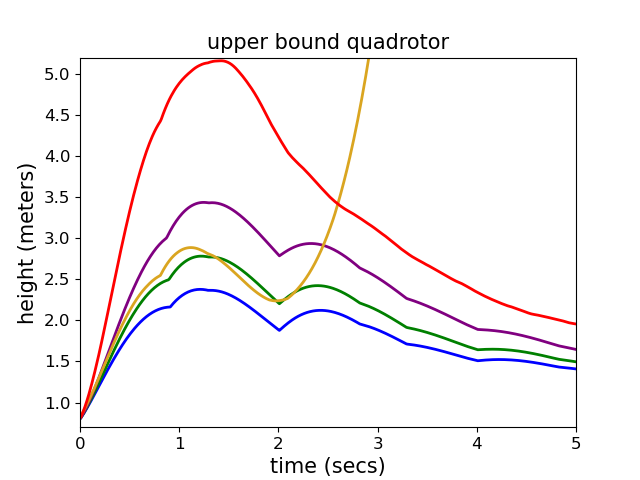
\includegraphics[scale = 0.39]{quadrotorImages/ubToolHeight.png}%\hspace{-2.2em}
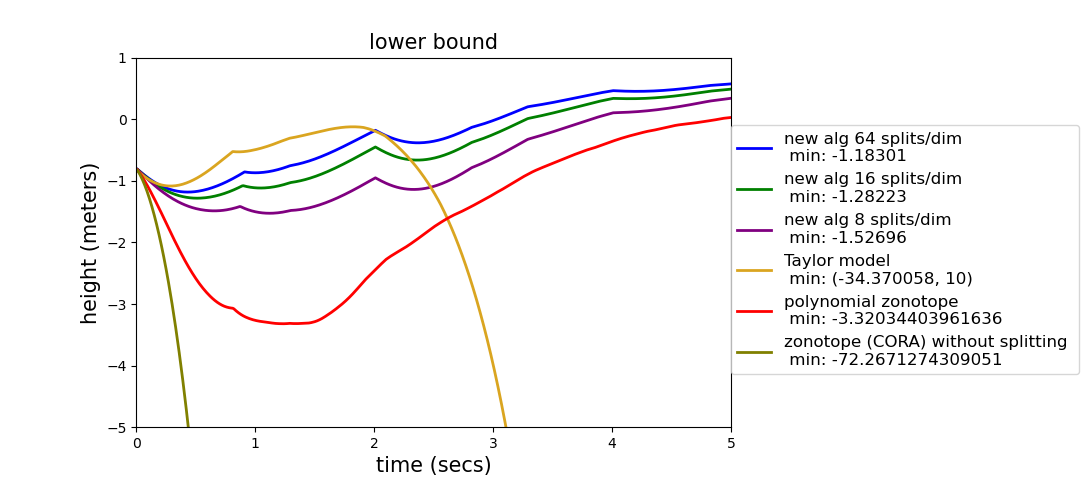
\includegraphics[scale = 0.39]{quadrotorImages/lbToolHeight.png}

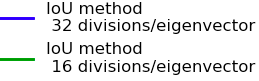
\includegraphics[scale = 0.41]{quadrotorImages/leg1.png}~
  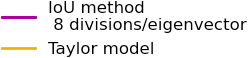
\includegraphics[scale = 0.41]{quadrotorImages/leg2.png}~
  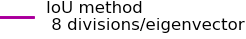
\includegraphics[scale = 0.41]{quadrotorImages/leg3.png}
\caption{Flowpipe bounds on height at different time points.\\
Note: Union method resulted in infinite bounds (not plotted).}\label{fig:flowquadrotor}
\end{figure}
% 
\subsection{$12$-dimensional model of quadrotor}
We consider the $12$-dimensional model of a quadrotor with three
inputs presented in the ARCH 2020 friendly
competition~\cite{geretti2020arch}, whose dynamics is given in the
appendix.  It has a $12$-dimensional state vector $x
= \rb{p_n,p_e,h,u,v,w,\phi,\theta,\psi,p,q,r}$, where $h$ is the
height of the quadrotor and a $3$-dimensional input vector $u
= \rb{u_1,u_2,u_2}$.  We take a larger initial set than the one given
in the competition~\cite{geretti2020arch} so that there is significant
linearization error in the flowpipe.  Our initial set in S.I. units
is $X_0 = [-0.8,0.8]^6\times[-0.5,0.5]^2\times[0,0]\times
[-1,1]^2\times[0,0]$.  The input set is $\rb{u_1,u_2,u_3}\in
[-0.99,1.01]\times[-0.01,0.01]^2$.  The goal of controller is to
stabilize the vertical height of the quadrotor at $h = 1\si{\meter}$.

%% \emph{Settings:}  The simulation time step is $\delta = 0.01\si{\second}$.  
%% For Flowstar Taylor model, the order of Taylor expansion is $7$.  For
%%   the CORA polynomial zonotope, generator order is $200$ and order of
%%   dependent generators is $2000$.  The zonotope order of our IoU
%%   method and the union method is $l=200$.  Also, $K = 20$ and
%%   $\epsilon = 10^{-12}$.  For the only union method, we take the
%%   normalization error $\rho$ as the Taylor error before division
%%   $\taylor{f}{X_0}{u}$.  We ran our IoU method and the union method on
%%   an AWS c5a.16xlarge cluster with 64 virtual cpus.  For Flowstar, we
%%   used AWS t2.large instance.  We ran CORA in MATLAB 2019a on the
%%   computer specified in the previous illustrative example.  The
%%   simulation time horizon is $[0, 5 s]$.
  
%% \is{The setting is mostly the same as the previous examples. Could we create a subsection on experimental setup before the examples and put these details there?}

\emph{Results:}  Our IoU method for each of the $8$, $16$ and $32$ divisions per
  eigenvector direction showed much higher accuracy than other
  methods.  The union method based on division using
  Equation~\ref{eqn:pi} resulted in very high linearization error and
  consequently infinite bounds $[-1,1]^{12}$ after $0.5 s$ simulation
  time, where the normalization error is taken to be $\rho
  = \taylor{f}{X_0}{u}$.  We plotted the flowpipe bounds for the
  height in Figure~\ref{fig:flowquadrotor}.  The figure clearly shows
  high increase in accuracy by using intersection of unions compared
  to other methods.  The computation times are given in
  Table~\ref{tab:comptimes}.  The preprocessing time before simulation
  for our IoU method is $44\si{\second}$.
%
